% ===================== HORIZON =====================
\subsection{HORIZON}\label{ds:horizon}
\naturalbadge\ \partialbadge\ \lbl{failure modes (LLM judge)}\ \lbl{step: web subset only}\ \lbl{single-agent}\ \lbl{WebArena / AgentBench-OS / BIRD / IsaacSim}

\begin{identity}
Paper & \emph{The Long-Horizon Task Mirage? Diagnosing Where and Why Agentic Systems Break} --- Wang et al.\ (UW--Madison / UC Berkeley; Mutlu, Song, Nowak), arXiv:2604.11978, Apr 2026 (preprint; ethics statement refers to COLM 2026) \cite{horizon2026}\\
Links & \href{https://huggingface.co/datasets/xwang2775/long-horizon-agent-failures}{HF \code{xwang2775/long-horizon-agent-failures}} (runs + judge labels, 19.5 GB, ungated, no card) \textperiodcentered\ \href{https://huggingface.co/datasets/xwang2775/horizon-tasks}{HF \code{xwang2775/horizon-tasks}} (task definitions, 786 rows, \emph{gated}) \textperiodcentered\ \href{https://xwang2775.github.io/horizon-leaderboard/}{leaderboard}\\
License & none stated on either HF repo or in the paper\\
Status & subset downloaded (187 MB of 19.5 GB): all judge bundles \code{result\_\{1,2,3,5\}/}, all \code{os/}, \code{database/}, \code{embodied/} raw runs and the web step logs; skipped the web Playwright traces and HTML page renders ($>$95\% of the volume). \code{horizon-tasks} access request denied; \code{data/horizon/hf/}\\
\end{identity}

\begin{multicols}{2}
\paragraph{Description} HORIZON is a \emph{diagnostic} benchmark for long-horizon agent tasks: it builds tasks of controllable horizon $s$ in four domains, runs single-agent systems on them and attributes every failure to one of seven failure modes with a trajectory-grounded \textbf{LLM-as-a-Judge}. It belongs to the MAST family (failure taxonomy, judge-labelled at scale) rather than to the human-annotated who/when benchmarks. Domains and base benchmarks:
\begin{itemize}
\item \textbf{Web} (WebArena shopping-admin / Postmill / GitLab; CoT agent on accessibility trees) and \textbf{Embodied} (bimanual IsaacSim 5.0, primitive-action plans): \emph{breadth} extension, $k$ base tasks joined by ``AND'' ($s{=}1\ldots5$);
\item \textbf{OS} (AgentBench-OS, bash ReAct agent) and \textbf{Database} (MAC-SQL on BIRD-style text-to-SQL): \emph{depth} extension, intermediate permission checks / filtering steps inserted (OS $s{=}1\ldots10$, DB $s{=}1\ldots8$).
\end{itemize}
``700+'' tasks; backbones GPT-5-mini and Claude-4-Sonnet (appendix figures say GPT-4o-mini / Claude-3.5-Sonnet --- an inconsistency); three OS runs per task set. Failures are natural. The environment verifier gives pass/fail; the judge independently reads the serialised trajectory and outputs \code{failure\_type} (\code{Success} or a mode) and a one-sentence \code{reason}; in the web/GPT-5-mini subset it also outputs a \code{failure\_step\_number} and a 5-step window summary. \textbf{Human validation} is limited to a 40-trajectory pilot: $\kappa$(human, human) = 0.61, $\kappa$(human, judge) = 0.84; those human labels are not released. \textbf{Taxonomy} (7 modes): Environment (acts on stale state), Instruction (ill-defined / partially understood), False Assumption, Planning Error (sub-plan / action) --- present at all horizons --- and Catastrophic Forgetting, History Error Accumulation, Memory Limitation --- predominantly long-horizon. The paper also splits them into process-level (72.5\%) vs design-level (27.5\%) failures.

\paragraph{Metrics and baselines} HORIZON benchmarks \emph{agents}, not attributors: success rate vs level $s$ with a ``break level'', and the failure-mode mix per domain/model. There is no attribution leaderboard --- the judge is the attribution method. Paper findings: web collapses at very small $s$, OS and DB degrade gradually, embodied steeply. Failure mix, paper (3,100+ trajectories, \%) vs released \code{result\_2} (counts):

\begin{center}\small
\begin{tabular}{@{}ll@{}}\toprule
Domain & \makecell[l]{paper, \% of failures\\release \code{result\_2}, counts}\\\midrule
Web & \makecell[l]{Plan 74.9, Env 11.3, Mem 6.2\\Plan 351, Env 27, FA 25, CF 22}\\\addlinespace[2pt]
OS & \makecell[l]{Plan 36.7, Instr 25.9, Env 17.3, Mem 15.1\\CF 717, Plan 545, Instr 503, Env 34}\\\addlinespace[2pt]
Database & \makecell[l]{Plan 79.3\\Plan 90, Instr 13, FA 10}\\\addlinespace[2pt]
Embodied & \makecell[l]{Plan 94.9\\Plan 139, Instr 5, FA 3}\\\bottomrule
\end{tabular}
\end{center}
The released pass contains \emph{no} Memory Limitation label and 29.6\% Catastrophic Forgetting, so the paper's figures come from a different judge pass. By model (paper): GPT failures 64.9\% Planning / 18.3\% Memory; Claude failures 32.5\% Environment / 16.5\% Instruction.

\paragraph{Schema} \code{result\_2/classified\_results.json} is the main judge output: 3,782 records with \code{id} (e.g.\ \code{web\_gpt\_5\_mini\_step\_4\_6}, \code{os\_gpt\_run\_0\_aug-cf3-007-\ldots}, \code{db\_gpt\_39}, \code{embodied\_claude\_<ULID>}), \code{domain}, \code{model} (\code{gpt} / \code{claude}), \code{run} (level), \code{passed} or \code{score} (environment verdict; present for 3,512), \code{trajectory} (domain-specific text: web \code{[Step n]} blocks with \code{Page}/\code{Agent}/\code{Action}; OS alternating \code{[Agent]}/\code{[OS response]}; DB one block with predicted vs gold SQL; embodied a primitive plan), \code{failure\_type}, \code{reason}. \code{result\_3/} is a second full judge pass over the same ids, \code{result\_1/} an earlier 1,499-record pass, and \code{result\_5/} the web/GPT-5-mini pass (371 records) adding \code{failure\_step\_number} and \code{steps} (judge's \code{label}/\code{summary}/\code{raw} for the last $\le$5 steps). Raw runs: \code{os/run\_\{0,1,2\}/<model>/<level>/runs.jsonl} (AgentBench format), \code{database/analyzed\_results\_final\_\{gpt,claude\}.json}, \code{embodied/<model>/<ULID>.json}, and one directory per web level, \code{web/<model>/} \code{5\_mini\_step\_<s>/}, with \code{config.json}, \code{steps\_*.txt}, \code{failure\_analysis.json} (an earlier per-task judge output) and \code{traces/*.zip}.
\end{multicols}

\paragraph{Statistics} computed from the downloaded \code{result\_2} (main pass) and \code{result\_5} (step labels); paper-only numbers marked.\par\nobreak\vspace{1pt}
\noindent\begin{minipage}[t]{0.56\linewidth}\vspace{0pt}\small\setlength{\tabcolsep}{4pt}
\begin{tabular}{@{}lrrrrr@{}}\toprule
 & All & OS & Web & Embod. & DB\\\midrule
trajectories (release) & 3,782 & 2,735 & 597 & 270 & 180\\
judge: fail / success & 2,498 / 1,284 & 1,811 / 924 & 427 / 170 & 147 / 123 & 113 / 67\\
GPT / Claude & 1,740 / 2,042 & 1,366 / 1,369 & 149 / 448 & 135 / 135 & 90 / 90\\
steps: mean / median & 13.7 / 11 & 12.7 / 11 & 23.5 / 10 & 9.8 / 9 & 1\\
steps: max & 151 & 50 & 151 & 34 & 1\\
step-level labels & 294 & --- & 294 & --- & ---\\\bottomrule
\end{tabular}

\smallskip Paper counts differ: 3,132 trajectories (web 767, OS 2,146, DB 84, embodied 135), 1,995 failures (paper). Characters per trajectory: mean 6.7\,k, median 5.4\,k, max 103\,k (web p90 39\,k). Environment verdict vs judge disagree on 12.9\% of runs where both exist (200 env-passes labelled failure, 252 env-fails labelled \code{Success}). Judge self-consistency (\code{result\_2} vs \code{result\_3}): exact label 77.5\%, success-vs-failure 94.3\%, category given both fail 73.3\% (main confusions CF$\leftrightarrow$Planning, Instruction$\leftrightarrow$Planning). \code{result\_5} (web/GPT, 294 labelled failures): Planning 252, Environment 17, History Error Accumulation 10, Instruction 8, False Assumption 7, Memory Limitation 5; error step mean 9.5, median 6, max 61; relative position mean 0.44, median 0.42 (49 of 294 in the first decile).
\end{minipage}\hfill
\begin{minipage}[t]{0.42\linewidth}\vspace{0pt}
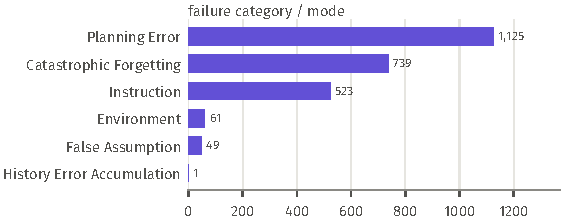
\includegraphics[width=\linewidth]{figures/cat_horizon.pdf}\\[2pt]
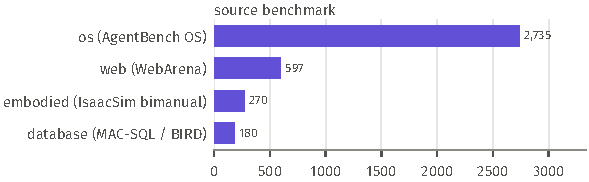
\includegraphics[width=\linewidth]{figures/bench_horizon.pdf}
\end{minipage}

\paragraph{Example trajectory} \code{web\_gpt\_5\_mini\_step\_4\_6} from \code{result\_5} (WebArena shopping-admin, GPT-5-mini, breadth level $s{=}4$; 14 steps; environment score 0). The agent sees at step 2 that order 299 is already cancelled, starts the bestsellers report, then at step 9 forgets this and goes back to cancel the order, loops on the same search and early-stops. Label (\emph{Memory Limitation}, step 9) and reason come from the LLM judge, not a human.
% auto-generated by scripts/render_traj.py -- do not edit
\trajtask{web\_gpt\_5\_mini\_step\_4\_6}{Cancel order 299 AND What is the top-1 best-selling product in 2022 AND Show all customers AND Get the billing name of the oldest complete order}
\begin{trajstep}{1}{web agent (gpt-5-mini)}{agA}
Observation:\allowbreak{} Tab 0 (current):\allowbreak{} Dashboard /\allowbreak{} Magento Admin\newline Thought:\allowbreak{} Let's think step-by-step. I will open the order row for order 299 to cancel it.\par In summary,\allowbreak{} the next action I will perform is ```click [975]```\newline Action:\allowbreak{} click [975] where [975] is [975] row 'http:\allowbreak{}/\allowbreak{}/\allowbreak{}localhost:\allowbreak{}7780/\allowbreak{}admin/\allowbreak{}sales/\allowbreak{}order/\allowbreak{}view/\allowbreak{}order\_id/\allowbreak{}299/\allowbreak{}'
\end{trajstep}
\begin{trajstep}{2}{web agent (gpt-5-mini)}{agA}
Observation:\allowbreak{} Tab 0 (current):\allowbreak{} \#000000299 /\allowbreak{} Orders /\allowbreak{} Operations /\allowbreak{} Sales /\allowbreak{} Magento Admin\newline Thought:\allowbreak{} Let's think step-by-step.\par The order view shows Order Status =\allowbreak{} "Canceled",\allowbreak{} so order 299 is already canceled. Next I need the top-1 best-selling product in 2022,\allowbreak{} show all customers,\allowbreak{} and get the billing name of the oldest "Complete" order. I'll navigate to the Reports section to find sales/\allowbreak{}bestsellers.\par In summary,\allowbreak{} the next action I will perform is ```click [1322]```\newline Action:\allowbreak{} click [1322] where [1322] is [1322] link '\textbackslash{}ue60a REPORTS'
\end{trajstep}
\begin{trajstep}{3}{web agent (gpt-5-mini)}{agA}
Observation:\allowbreak{} Tab 0 (current):\allowbreak{} \#000000299 /\allowbreak{} Orders /\allowbreak{} Operations /\allowbreak{} Sales /\allowbreak{} Magento Admin\newline Thought:\allowbreak{} Let's think step-by-step. The order view shows Order 299's status is already "Canceled",\allowbreak{} so no further action is needed to cancel it. Next,\allowbreak{} I'll open the Bestsellers report to find the top-selling product for 2022.\par In summary,\allowbreak{} the next action I will perform is ```click [2280]```\newline Action:\allowbreak{} click [2280] where [2280] is [2280] link 'Bestsellers'
\end{trajstep}
\begin{trajstep}{4}{web agent (gpt-5-mini)}{agA}
Observation:\allowbreak{} Tab 0 (current):\allowbreak{} Bestsellers Report /\allowbreak{} Products /\allowbreak{} Reports /\allowbreak{} Magento Admin\newline Thought:\allowbreak{} I will set the report's date range to 2022. In summary,\allowbreak{} the next action I will perform is ```type [4573] [01/\allowbreak{}01/\allowbreak{}2022] [0]```\newline Action:\allowbreak{} type [4573] [01/\allowbreak{}01/\allowbreak{}2022] where [4573] is [4573] textbox 'From *' required:\allowbreak{} True
\end{trajstep}
\begin{trajstep}{5}{web agent (gpt-5-mini)}{agA}
Observation:\allowbreak{} Tab 0 (current):\allowbreak{} Bestsellers Report /\allowbreak{} Products /\allowbreak{} Reports /\allowbreak{} Magento Admin\newline Thought:\allowbreak{} Let's think step-by-step. I will enter the end date for the report so I can run the 2022 bestsellers report.\par In summary,\allowbreak{} the next action I will perform is ```type [4576] [12/\allowbreak{}31/\allowbreak{}2022] [1]```\newline Action:\allowbreak{} type [4576] [12/\allowbreak{}31/\allowbreak{}2022 ] where [4576] is [4576] textbox 'To *' required:\allowbreak{} True
\end{trajstep}
\begin{trajstep}{6}{web agent (gpt-5-mini)}{agA}
Observation:\allowbreak{} Tab 0 (current):\allowbreak{} Bestsellers Report /\allowbreak{} Products /\allowbreak{} Reports /\allowbreak{} Magento Admin\newline Thought:\allowbreak{} Let's think step-by-step. First I will generate the bestsellers report for 2022 to find the top-1 product.\par In summary,\allowbreak{} the next action I will perform is ```click [4782]```\newline Action:\allowbreak{} click [4782] where [4782] is [4782] button 'Show Report'
\end{trajstep}
\begin{trajstep}{7}{web agent (gpt-5-mini)}{agA}
Observation:\allowbreak{} Tab 0 (current):\allowbreak{} Bestsellers Report /\allowbreak{} Products /\allowbreak{} Reports /\allowbreak{} Magento Admin\newline Thought:\allowbreak{} Let's think step-by-step. The best-sellers report results need to be displayed to identify the top product for 2022. I'll (re)run the report by clicking the "Show Report" button.\par In summary,\allowbreak{} the next action I will perform is ```click [6091]```\newline Action:\allowbreak{} click [6091] where [6091] is [6091] button 'Show Report'
\end{trajstep}
\begin{trajstep}{8}{web agent (gpt-5-mini)}{agA}
Observation:\allowbreak{} Tab 0 (current):\allowbreak{} Bestsellers Report /\allowbreak{} Products /\allowbreak{} Reports /\allowbreak{} Magento Admin\newline Thought:\allowbreak{} In summary,\allowbreak{} the next action I will perform is ```click [9442]```\newline Action:\allowbreak{} click [9442] where [9442] is [9442] link '\textbackslash{}ue60b SALES'
\end{trajstep}
\begin{faultystep}{9}{web agent (gpt-5-mini)}{agA}
Observation:\allowbreak{} Tab 0 (current):\allowbreak{} Bestsellers Report /\allowbreak{} Products /\allowbreak{} Reports /\allowbreak{} Magento Admin\newline Thought:\allowbreak{} Let's think step-by-step. To cancel order \#299 I need to open the Orders list under Sales. The Orders link is available in the Sales menu.\par In summary,\allowbreak{} the next action I will perform is ```click [9650]```\newline Action:\allowbreak{} click [9650] where [9650] is [9650] link 'Orders'
\end{faultystep}
\begin{trajstep}{10}{web agent (gpt-5-mini)}{agA}
Observation:\allowbreak{} Tab 0 (current):\allowbreak{} Orders /\allowbreak{} Operations /\allowbreak{} Sales /\allowbreak{} Magento Admin\newline Thought:\allowbreak{} Let's think step-by-step. To cancel order \#299 I should locate it in the Orders list --- the page has a "Search by keyword" box. I'll search for "299" to load that order.\par In summary,\allowbreak{} the next action I will perform is ```type [12939] [299] [1]```\newline Action:\allowbreak{} type [12939] [299 ] where [12939] is [12939] textbox 'Search by keyword' required:\allowbreak{} False
\end{trajstep}
\begin{trajstep}{11}{web agent (gpt-5-mini)}{agA}
Observation:\allowbreak{} Tab 0 (current):\allowbreak{} Orders /\allowbreak{} Operations /\allowbreak{} Sales /\allowbreak{} Magento Admin\newline Thought:\allowbreak{} Let's think step-by-step. I will first run the search for the order so I can cancel it.\par In summary,\allowbreak{} the next action I will perform is ```click [12940]```\newline Action:\allowbreak{} click [12940] where [12940] is [12940] button 'Search'
\end{trajstep}
\begin{trajstep}{12}{web agent (gpt-5-mini)}{agA}
Observation:\allowbreak{} Tab 0 (current):\allowbreak{} Orders /\allowbreak{} Operations /\allowbreak{} Sales /\allowbreak{} Magento Admin\newline Thought:\allowbreak{} In summary,\allowbreak{} the next action I will perform is ```type [12939] [299] [1]```\newline Action:\allowbreak{} type [12939] [299 ] where [12939] is [12939] textbox 'Search by keyword' required:\allowbreak{} False
\end{trajstep}
\begin{trajstep}{13}{web agent (gpt-5-mini)}{agA}
Observation:\allowbreak{} Tab 0 (current):\allowbreak{} Orders /\allowbreak{} Operations /\allowbreak{} Sales /\allowbreak{} Magento Admin\newline Thought:\allowbreak{} Let's think step-by-step. I will replace the current search keyword with the order ID "299" and submit the search to locate the order.\par In summary,\allowbreak{} the next action I will perform is ```type [12939] [299] [1]```\newline Action:\allowbreak{} type [12939] [299 ] where [12939] is [12939] textbox 'Search by keyword' focused:\allowbreak{} True required:\allowbreak{} False
\end{trajstep}
\begin{trajstep}{14}{web agent (gpt-5-mini)}{agA}
Observation:\allowbreak{} Tab 0 (current):\allowbreak{} Orders /\allowbreak{} Operations /\allowbreak{} Sales /\allowbreak{} Magento Admin\newline Thought:\allowbreak{}\newline Action:\allowbreak{} stop [Early stop:\allowbreak{} Same typing action for 3 times]
\end{trajstep}
\trajannotation{web agent (single-agent)}{9}{Memory Limitation}{After noting in Step 2 that order 299 was already canceled,\allowbreak{} the agent later forgot this and attempted to cancel it again (Step 9),\allowbreak{} repeating search actions instead of proceeding with the remaining tasks.}{Canceled}{Early stop:\allowbreak{} Same typing action for 3 times}{\textbf{domain}: web; \textbf{model}: gpt; \textbf{run}: 5\_mini\_step\_4; \textbf{task\_id}: 6; \textbf{score}: 0.0; \textbf{judge}: LLM-as-a-Judge (trajectory-grounded),\allowbreak{} not human; \textbf{judge\_step\_window\_summaries}: [\{"label":\allowbreak{} "establishment step",\allowbreak{} "summary":\allowbreak{} "Agent observes order 299 is already canceled and plans to work on other tasks.",\allowbreak{} "raw":\allowbreak{} "[Step 2]\textbackslash{}nPage :\allowbreak{} Tab 0 (current):\allowbreak{} \#000000299 /\allowbreak{} Orders /\allowbreak{} Operations /\allowbreak{} Sales /\allowbreak{} Magento Admin\textbackslash{}nAgent:\allowbreak{} Let's think step-by-step.\textbackslash{}n\textbackslash{}nThe order view shows Order Status =\allowbreak{} \textbackslash{}"Canceled\textbackslash{}",\allowbreak{} so order 299 is already canceled. Next I need th\newline [...] (2,\allowbreak{}070 chars omitted) [...]\newline it.\textbackslash{}n\textbackslash{}nIn summary,\allowbreak{} the next action I will perform is ```click [12940]```\textbackslash{}nAction:\allowbreak{} click [12940] where [12940] is [12940] button 'Search'"\}]}


\paragraph{Notes} (i) Unique: controllable horizon --- the same base task reappears at increasing depth/breadth, so failure modes can be plotted against horizon; four heterogeneous domains including embodied manipulation and text-to-SQL; two full judge passes allow measuring judge self-consistency. (ii) \textbf{Labels are LLM-generated}: treat HORIZON as a judge-labelled taxonomy dataset (like MAST-Data), validated on 40 human-checked trajectories whose labels are not released; step labels exist only for 294 web/GPT runs and are judge outputs. (iii) Granularity varies by domain: database ``trajectories'' are one predicted-vs-gold SQL, embodied ones are plans without observations; step-level attribution is only meaningful for web and OS. (iv) Inconsistencies: release 3,782 vs paper 3,132 trajectories; released mode mix (0 Memory Limitation, 29.6\% Catastrophic Forgetting) vs paper (15\% Memory Limitation on OS); backbone names differ between main text and appendix; no license; the HF viewer fails on the repo. (v) Volume is misleading: $>$95\% of the 19.5 GB are Playwright zips and page renders; the attribution JSON is $\approx$140 MB. (vi) Overlaps: base tasks from WebArena, AgentBench-OS and BIRD --- none shared with the MAS attribution datasets; conceptually closest to MAST and AgentErrorBench.
